\documentclass{article}
\iffalse
This file is protected by Copyright. Please refer to the COPYRIGHT file
distributed with this source distribution.

This file is part of OpenCPI <http://www.opencpi.org>

OpenCPI is free software: you can redistribute it and/or modify it under the
terms of the GNU Lesser General Public License as published by the Free Software
Foundation, either version 3 of the License, or (at your option) any later
version.

OpenCPI is distributed in the hope that it will be useful, but WITHOUT ANY
WARRANTY; without even the implied warranty of MERCHANTABILITY or FITNESS FOR A
PARTICULAR PURPOSE. See the GNU Lesser General Public License for more details.

You should have received a copy of the GNU Lesser General Public License along
with this program. If not, see <http://www.gnu.org/licenses/>.
\fi

\author{} % Force author to be blank
%----------------------------------------------------------------------------------------
% Paper size, orientation and margins
%----------------------------------------------------------------------------------------
\usepackage{geometry}
\geometry{
	letterpaper,			% paper type
	portrait,				% text direction
	left=.75in,				% left margin
	top=.75in,				% top margin
	right=.75in,			% right margin
	bottom=.75in			% bottom margin
 }
%----------------------------------------------------------------------------------------
% Header/Footer
%----------------------------------------------------------------------------------------
\usepackage{fancyhdr} \pagestyle{fancy} % required for fancy headers
\renewcommand{\headrulewidth}{0.5pt}
\renewcommand{\footrulewidth}{0.5pt}
\rhead{\small{ANGRYVIPER Team}}
%----------------------------------------------------------------------------------------
% Appendix packages
%----------------------------------------------------------------------------------------
\usepackage[toc,page]{appendix}
%----------------------------------------------------------------------------------------
% Defined Commands & Renamed Commands
%----------------------------------------------------------------------------------------
\renewcommand{\contentsname}{Table of Contents}
\renewcommand{\listfigurename}{List of Figures}
\renewcommand{\listtablename}{List of Tables}
\newcommand{\todo}[1]{\textcolor{red}{TODO: #1}\PackageWarning{TODO:}{#1}} % To do notes
\newcommand{\code}[1]{\texttt{#1}} % For inline code snippet or command line
%----------------------------------------------------------------------------------------
% Various pacakges
%----------------------------------------------------------------------------------------
\usepackage{hyperref} % for linking urls and lists
\usepackage{graphicx} % for including pictures by file
\usepackage{listings} % for coding language styles
\usepackage{rotating} % for sideways table
\usepackage{pifont}   % for sideways table
\usepackage{pdflscape} % for landscape view
%----------------------------------------------------------------------------------------
% Table packages
%----------------------------------------------------------------------------------------
\usepackage{tabularx} % c=center,l=left,r=right,X=fill
\usepackage{float}
\floatstyle{plaintop}
\usepackage[tableposition=top]{caption}
\newcolumntype{P}[1]{>{\centering\arraybackslash}p{#1}}
\newcolumntype{M}[1]{>{\centering\arraybackslash}m{#1}}
%----------------------------------------------------------------------------------------
% Block Diagram / FSM Drawings
%----------------------------------------------------------------------------------------
\usepackage{tikz}
\usetikzlibrary{shapes,arrows,fit,positioning}
\usetikzlibrary{automata} % used for the fsm
%----------------------------------------------------------------------------------------
% Colors Used
%----------------------------------------------------------------------------------------
\usepackage{colortbl}
\definecolor{blue}{rgb}{.7,.8,.9}
\definecolor{ceruleanblue}{rgb}{0.16, 0.32, 0.75}
\definecolor{drkgreen}{rgb}{0,0.6,0}
\definecolor{deepmagenta}{rgb}{0.8, 0.0, 0.8}
\definecolor{cyan}{rgb}{0.0,0.6,0.6}
\definecolor{maroon}{rgb}{0.5,0,0}
%----------------------------------------------------------------------------------------
% Update the docTitle and docVersion per document
%----------------------------------------------------------------------------------------
\def\docTitle{Component Data Sheet}
\def\docVersion{1.1}
%----------------------------------------------------------------------------------------
\date{Version \docVersion} % Force date to be blank and override date with version
\title{\docTitle}
\lhead{\small{\docTitle}}

\def\comp{zero\_pad}
\edef\ecomp{zero_pad}
\def\Comp{Zero Pad}
\graphicspath{ {figures/} }

\begin{document}

\section*{Summary - \Comp}
\begin{tabular}{|c|M{13.5cm}|}
	\hline
	\rowcolor{blue}
	                  &                        \\
	\hline
	Name              & \comp                  \\
	\hline
	Worker Type       & Application            \\
	\hline
	Version           & v1.3                  \\
	\hline
	Release Date      & February 2018           \\
	\hline
	Component Library & ocpi.assets.util\_comps \\
	\hline
	Workers           & \comp.hdl              \\
	\hline
	Tested Platforms  & xsim, isim, modelsim, Matchstiq-Z1(PL) \\
	\hline
\end{tabular}

\section*{Functionality}
\begin{flushleft}
	The \Comp{} component inputs samples and inserts a configurable number of zeros between output samples.
\end{flushleft}

\section*{Worker Implementation Details}
\begin{flushleft}
	In order to be maximally flexible, the component does not define input/output protocols explicitly. The input/output data widths are defined at build time, which in turn define the respective input/output sample sizes.\medskip
	
	The input and output data width are the same and are configurable via the \verb+DWIDTH_p+ parameter. All zeros inserted between samples are also of size \verb+DWIDTH_p+.\medskip
	
	The message size on the output is equal to the number of zeros inserted plus 1.
\end{flushleft}

\section*{Block Diagrams}
\subsection*{Top level}
\begin{center}
	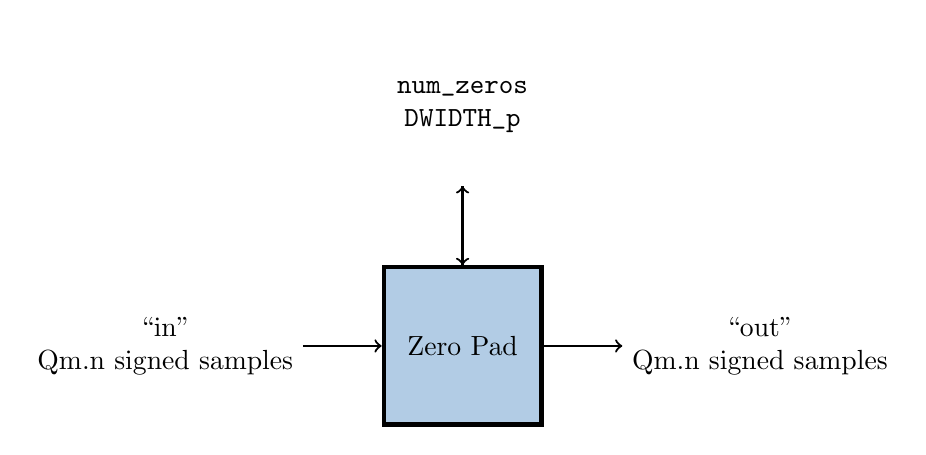
\begin{tikzpicture}[% List of styles applied to all, to override specify on a case-by-case
			every node/.style={
				align=center,  		% use this so that the "\\" for line break works
				minimum size=2cm	% creates space above and below text in rectangle
			},
			every edge/.style={draw,thick}
		]
		\node[rectangle,ultra thick,draw=black,fill=blue](R2){\Comp};
		\node[rectangle,draw=white,fill=white](R3)[left= of R2]{``in'' \\ Qm.n signed samples};
		\node[rectangle,draw=white,fill=white](R4)[right= of R2]{``out'' \\ Qm.n signed samples};
		\node[rectangle,draw=white,fill=white](R5)[above= of R2]{\verb+num_zeros+\\\verb+DWIDTH_p+};
		\path[->]
		(R3)edge []	node [] {} (R2)
		(R2)edge []	node [] {} (R4)
		(R2)edge []	node [] {} (R5)
		(R5)edge []	node [] {} (R2)
		;
	\end{tikzpicture}
\end{center}

\section*{Source Dependencies}
\subsection*{\comp.hdl}
\begin{itemize}
	\item ocpiassets/components/util\_comps/\comp.hdl/\comp.vhd
\end{itemize}
\subsection*{\comp.rcc}
\begin{itemize}
	\item ocpiassets/components/util\_comps/\comp.rcc/\comp.cc
\end{itemize}
\begin{landscape}
	\section*{Component Spec Properties}
	\begin{scriptsize}
		\begin{tabular}{|p{2cm}|p{1.5cm}|c|c|c|p{1.5cm}|p{1cm}|p{7cm}|}
			\hline
			\rowcolor{blue}
			Name          		& Type  & SequenceLength & ArrayDimensions & Accessibility       & Valid Range & Default & Usage              	\\
			\hline
			\verb+DWIDTH_p+ 	& ULong & -              & -               & Readable, Parameter & 8,16,32,64  & 16      & Input and output port data width\\
			\hline
			\verb+num_zeros+  	& Short & -              & M\_p            & Readable, Writable	 & Standard    & -       & Number of zeros to be inserted between output samples \\
			\hline
		\end{tabular}
	\end{scriptsize}

	\section*{Worker Properties}
	There are no worker implementation-specific properties for this component 

	\section*{Component Ports}
	\begin{scriptsize}
		\begin{tabular}{|M{2cm}|M{1.5cm}|M{4cm}|c|c|p{9cm}|}
			\hline
			\rowcolor{blue}
			Name & Producer & Protocol			& Optional & Advanced 					& Usage      			\\
			\hline
			in   & false    & -					& false    & -        					& Signed real samples  	\\
			\hline
			out  & true     & - 				& false    & -							& Signed real samples	\\
			\hline
		\end{tabular}
	\end{scriptsize}
	\section*{Worker Interfaces}
	\subsection*{\comp.hdl}
	\begin{scriptsize}
		\begin{tabular}{|M{2cm}|M{1.5cm}|c|c|p{12cm}|}
			\hline
			\rowcolor{blue}
			Type            & Name & DataWidth 		& Advanced  & Usage                 \\
			\hline
			StreamInterface & in   & DWIDTH\_p		& - 		& Signed real samples 	\\
			\hline
			StreamInterface & out  & DWIDTH\_p		& -			& Signed real samples 	\\
			\hline
		\end{tabular}
	\end{scriptsize}
\end{landscape}

\section*{Control Timing and Signals}
\begin{flushleft}
	The \Comp{} HDL worker uses the clock from the Control Plane and standard Control Plane signals.\\
\end{flushleft}

\section*{Performance and Resource Utilization}
\subsubsection*{\comp.hdl}
\input{../../\ecomp.hdl/utilization.inc}
\section*{Test and Verification}
\begin{flushleft}
	Data widths of 8/16/32/64 are supported and fully tested on both RCC and HDL worker implementations. These widths combinations are tested with \verb+num_zeros+ equal to 0, 7, 8, 38, 127, and 255.\medskip

	Input data is generated by a python script with an input parameter that defines the number of 32-bit words to produce. The input file consists of a repeating pattern of 0x0123456789ABCDEF. The number of 32-bit words for each test case is 2048, which results in 1024 64-bit samples, 2048 32-bit samples, 4096 16-bit samples, or 8192 8-bit samples. Thus for each test case the 64-bit test pattern is repeated 1024 times to produce a file of 65,536 bits (or 8192 bytes).\medskip

	The \Comp{} component inputs each sample and \verb+num_zeros+ zeros are inserted between each output sample.\medskip

	For verification, the output file is first checked that the data is not all zero, and is then checked for the expected length. Once these quick checks are made the output data is compared against expected results sample-by-sample without use of any gold files.
\end{flushleft}
\end{document}
